\section{The Javadoc Tags}\label{sec:JavaDocTags}
The Javadoc\index{javadoc} tool comes with a set of tags that help to create compile documentation comments that generate neatly to a useful documentation of the product.

\Java also provides an API for custom tags  \autocite{ORACLE_DOC_TAGLET_INTERFACE}; it even provides an API  \autocite{ORACLE_DOC_DOCLET_PACKAGE,ORACLE_DOC_DOCLET_INTERFACE} that allows to customize the complete generation process.

%------------------------------------------------------------------------------

\subsection{The Standard Doclet Tags}
Most of the contents of this chapter is quoted from the document \bdq{JavaDoc Documentation Comment Specification for the Standard Doclet (JDK 25)} \autocite{ORACLE_DOC_JAVADOC_TAG}. 

The output of the Javadoc\index{javadoc} tool is determined by the implementation of the interface \lstinline|jdk.javadoc.doclet.Doclet| \autocite{ORACLE_DOC_DOCLET_INTERFACE} that is specified on the command line for \texttt{javadoc} by the options \texttt{-doclet} and \texttt{-docletpath} \autocite{ORACLE_TOOL:javadoc:options}. The \lstinline|Doclet| implementation is also responsible for interpreting the content of the documentation comments.

If no explicit \lstinline|Doclet| class is specified on the command line, the standard doclet (provided through the class \lstinline|jdk.javadoc.doclet.StandardDoclet| \autocite{ORACLE_DOC_STANDARDDOCLET_CLASS}) is used; it understands the Javadoc tags described below, and it provides an API for additional tags.

Alternative implementations for the \lstinline|Doclet| interface may accept the same syntax as the standard doclet, they may handle the tags completely different or they can ignore them completely. However, due to the support by many tools, the syntax supported by the standard doclet has become a \textit{de facto} standard.

%--------------------------------------------------------------------

\paragraph{\lstinline|@author|}\label{sec:TagAuthor}\index{author@"@author} Usage: \lstinline|@author <name-text>|

The tag adds an \bdq{\textsf{Author:}} entry with the specified name to the generated documentation when the \texttt{-author} option is specified on the command line for the Javadoc\index{javadoc}. A documentation comment can contain multiple \nameref{sec:TagAuthor} tags. Consider to use the custom \bdq{\nameref{sec:TagExtAuthor}}\index{extauthor@"@extauthor}  tag instead.

%--------------------------------------------------------------------

\paragraph{\lstinline|@code|}\label{sec:TagCode}\index{code@"@code}  Usage: \lstinline|{@code <text>}|

This is equivalent to \lstinline|<code>{@literal text}</code>|.

It displays text in the code font without interpreting the text as HTML\index{HTML} markup or nested Javadoc tags. This enables you to use regular angle brackets (\bdq{\textless} and \bdq{\textgreater}) instead of the HTML\index{HTML} entities (\texttt{\&lt;} and \texttt{\&gt;}) in documentation comments, such as in parameter types (\texttt{<Object>}), inequalities ($3 < 4$), or arrows (\texttt{-\textgreater}).

Use the \bdq{\{\nameref{sec:TagLiteral} …\}}\index{literal@"@literal} tag if you want the same functionality without the code font. 

%--------------------------------------------------------------------

\paragraph{\lstinline|@deprecated|}\index{deprecated@"@deprecated}  Usage: \lstinline|@deprecated <text>|

This tag is used in conjunction with the \lstinline|@Deprecated| \autocite{ORACLE_DOC_DEPRECATED_ANNOTATION} annotation to indicate that this API should no longer be used (even though it may continue to work).

The first sentence of the text should tell the user when the API was deprecated and what to use as a replacement. Subsequent sentences can also explain why it was deprecated.

A \bdq{\{\nameref{sec:TagLink} …\}}\index{link@"@link} tag that points to the replacement API should be added where feasible.


%--------------------------------------------------------------------

\paragraph{\lstinline|@docRoot|}  Usage: \lstinline|{@docRoot}|

Represents the relative path to the generated document's (destination) root directory from any generated page. This tag is useful when you want to include a file, such as a copyright page or company logo, that you want to reference from all generated pages.

%--------------------------------------------------------------------

\paragraph{\lstinline|@exception|} This is a synonym for the \bdq{\nameref{sec:TagThrows}}\index{throws@"@throws} tag; it should not be used.

%--------------------------------------------------------------------

\paragraph{\lstinline|@hidden|}\index{hidden@"@hidden}  Usage: \lstinline|@hidden|

Hides a program element from the generated API documentation. This tag may be used when it is not otherwise possible to design the API in a way that such items do not appear at all.

%--------------------------------------------------------------------

\paragraph{\lstinline|@index|}\index{index@"@index}  Usage: \lstinline|{@index <word> <description>}| or\\  
\lstinline|    {@index "<phrase>"  <description>}|

Declares that a word or phrase, together with an optional short description, should appear in the index files generated by the standard doclet. The index entry will be linked to the word or phrase that will appear at this point in the generated documentation. The description may be used when the word or phrase to be indexed is not clear by itself, such as for an acronym.

%--------------------------------------------------------------------

\paragraph{\lstinline|@inheritDoc|}\label{sec:TagInheritDoc}  Usage: \lstinline|{@inheritDoc}|

Inherits (copies) the documentation comment from the nearest inheritable class or implementable interface into the current documentation comment at this tag's location. This enables you to write more general comments higher up the inheritance tree and to write around the copied text.

\paragraph{\lstinline|@link|}\label{sec:TagLink}  Usage: \lstinline|{@link <module/package.class#member> <label>}|

Inserts an inline link with a visible text label that points to the documentation for the specified module, package, class, or member name of a referenced class. 

This tag is similar to the \nameref{sec:TagSee} tag. Both tags require the same references and accept the same syntax for \verb|<module/package.class#member>| and the label. The main difference is that the \lstinline|{@link}| tag generates an inline link rather than placing the link in the “See Also” section. The \lstinline|{@link}| tag begins and ends with curly braces to separate it from the rest of the inline text. If you need to use the right curly brace (“\}”) inside the label, then use the HTML entity notation \verb|&#125;|.

\paragraph{\lstinline|@linkplain|}\label{sec:TagLinkplain}  Usage: \lstinline|{@linkplain <module/package.class#member> <label>}|

Behaves the same as the \nameref{sec:TagLink} tag, except the link label is displayed in plain text rather than code font. Useful when the label is plain text.

\paragraph{\lstinline|@literal|}\label{sec:TagLiteral}  Usage: \lstinline|{@literal <text>}| 

Same as the \nameref{sec:TagCode} tag, but the text is shown as plain text and not in the code font.

\paragraph{\lstinline|@param|}\label{sec:TagParam}  Usage: \lstinline|@param <parameter-name> <description>|

Adds a parameter with the specified parameter name followed by the specified description to the “Parameters” section. The parameter name can be the name of a parameter in a method or constructor, or the name of a type parameter of a class, method, or constructor. Use angle brackets (“\verb#<…>#”) around such a parameter name to indicate the use of a type parameter.

\paragraph{\lstinline|@provides|}\label{sec:TagProvides}  Usage: \lstinline|@provides <service-type> <description>|

This tag may only appear in the documentation comment inside a \verb#module-info.java# file. It serves to document an implementation of a service that is provided by the module. The description may be used to specify how to obtain an instance of this service provider, and any important characteristics of the provider itself. 

\paragraph{\lstinline|@return|}\label{sec:TagReturn}  Usage: \lstinline|@return <description>|

Adds a “Returns” section with the description text to the documentation comment of a method.

\paragraph{\lstinline|@see|}\label{sec:TagSee}  Adds a “See Also” heading with a link or text entry that points to a reference. The \lstinline|@see| tag has three variations; see \autocite{ORACLE_DOC_JAVADOC_TAG} for the details.

\paragraph{\lstinline|@serial|}\label{sec:TagSerial} Used in the documentation comment for a default serializable field. See “Documenting Serializable Fields and Data for a Class”\autocite{ORACLE_DOC_OBJECT_SERIALIZATION:DocumentingSerializableFieldsData}. 

\paragraph{\lstinline|@since|}\label{sec:TagSince}  Usage: \lstinline|@since <since-text>|

Adds a “Since” heading with the specified \verb#<since-text># value to the generated documentation. The text has no special internal structure. This tag that this change or feature has existed since the software release specified by the \verb#<since-text># value, for example: \lstinline|@since 1.5|.

Although it would possible to provide a date or something else, it is recommended to always use a version number with the \lstinline|@since| tag.

\paragraph{\lstinline|@summary|}\label{sec:TagSummary}  Usage:  \lstinline|{@summary <text>}|

Identifies  the summary of an API description, as an alternative to the default policy to identify and use the first sentence of the API description. The tag only has significance when used at the beginning of a description. In all cases, the tag is rendered by simply rendering its content.

The \lstinline|{@summary}| tag has to be used always when a documentation comment has more than one sentence; see also chapter \tqvref{sec:StructureAndContents}.

\paragraph{\lstinline|@throws|}\label{sec:TagThrows}  Usage: \lstinline|@throws <class-name> <description>|

The \lstinline|@throws| tag adds a “Throws” subheading to the generated documentation, with the \verb#<class-name># and the description text. The class name is the name of the exception that might be thrown by the method, and the description provides information about the conditions for that exception to be thrown. 

\paragraph{\lstinline|@uses|}\label{sec:TagUses}  Usage: \lstinline|@uses <service-type> <description>|

This tag may only appear in the documentation comment inside a \verb#module-info.java# file. It serves to document that a service may be used by the module. The description may be used to specify the characteristics of the service that may be required, and what the module will do if no provider for the service is available.

\paragraph{\lstinline|@value|}\label{sec:TagValue}  Usage: \lstinline|{@value}| or \lstinline|{@value <module/package.class#field>}|

This tag is used to display the values of constant in the generated documentation. When the \lstinline|{@value}| tag is used without an argument in the documentation comment of a \lstinline|static final| field, it displays the value of that constant:
\begin{lstlisting}
/**
 * The value of this constant is {@value}.
 */
public static final String SCRIPT_START = "<script>"
\end{lstlisting}

When used with the argument \verb|<module.package.class#field>| in any documentation comment, the \lstinline|{@value}>| tag displays the value of the specified constant:
\begin{lstlisting}
/**
 * Evaluates the script starting with {@value #SCRIPT_START}.
 */
public final String evalScript( String script ) { … }
\end{lstlisting}
The argument \verb|<module.package.class#field>| takes a form similar to that of the \nameref{sec:TagLink}, the \nameref{sec:TagLinkplain}, or the \nameref{sec:TagSee} tag argument, except that the member always must be a \lstinline|static final| field.

\paragraph{\lstinline|@version|}\label{sec:TagVersion}  Usage: \lstinline|@version <version-text>|

Adds a “Version” subheading with the specified \verb#<version-text># value to the generated documents when the \verb#-version# option is specified on the command line. This tag is intended to hold the current release number of the software that this code is part of, as opposed to the \nameref{sec:TagSince} tag, which holds the release number where this code was introduced. The \verb#<version-text># value has no special internal structure.

%==============================================================================
% End of file!!
%==============================================================================


\subsection{Custom Tags for JavaDoc}\label{sec:CustomTagsForJavaDoc}
The Javadoc\index{javadoc} tool allows to add custom tags that can be used within the documentation comments.

There are two different ways to add custom tags. The easier one is to configure them just on the command line for the tool, the more flexible one requires to write Java code that implements the \lstinline|jdk.javadoc.doclet.Taglet|\index{jdk.javadoc.doclet!Taglet} \autocite{ORACLE_DOC_TAGLET_INTERFACE} interface.

\subsubsection{Simple Custom Tags}\label{sec:SimpleCustomTags}
A simple custom tag is configured completely on the command line for the invocation of the Javadoc\index{javadoc} tool. This approach allows only block tag, but the text for these tags comes with full support for all inline tags.

\keeplisting{2}
The command line option for a new simple custom tag looks like this:
\begin{lstlisting}[numbers=none,language={}]
-tag <name>[:[<locations>]:<header>]
\end{lstlisting}

This specifies a custom block tag \texttt{<name>}. For the Javadoc\index{javadoc} tool to spell-check tag names, it is important to include a \texttt{-tag} option for every custom tag that is present in the source code, disabling (with \texttt{X} as the location) those that aren't being output in the current run.

\texttt{<locations>} is a combination of the letters below, in either uppercase or lowercase, that determine where the custom tag is allowed:
\begin{itemize}[nosep]
	\item{\texttt{A}: all declarations}
	\item{\texttt{C}: constructors\index{constructor}}
	\item{\texttt{F}: fields\index{field}}
	\item{\texttt{M}: methods\index{method}}
	\item{\texttt{O}: the overview page and other documentation files in doc-files subdirectories}
	\item{\texttt{P}: packages\index{package}}
	\item{\texttt{S}: modules\index{module}}
	\item{\texttt{T}: types (classes\index{class} and interfaces\index{interface})}
	\item{\texttt{X}: nowhere: the tag is disabled, and will be ignored, together with its argument}
\end{itemize}

Finally, \texttt{<header>} is the tag heading that is rendered in bold, followed by the tag's single argument in the next line.

\keeplisting{2}
For the command line option
\begin{lstlisting}[numbers=none,language={}]
-tag implNote:a:Implementation Note:
\end{lstlisting}
and the source code below
\keeplisting{10}
\begin{lstlisting}
/**
 *  {@summary Retrieves data from the queue.}
 *  
 *  @param  <T> The type of the data in the queue.
 *  @param  queue   The queue.
 *  @return An instance of
 *      {@link Optional}
 *      that holds the retrieved data.
 *  
 *  @implNote The method may not block; if the queue is (currently) empty,
 *      the implementation must return
 *      {@linkplain Optional#empty() empty}.
 */
public <T> T retrieveData( final Queue<T> queue );
\end{lstlisting}
the output will look like this:
\begin{center}
	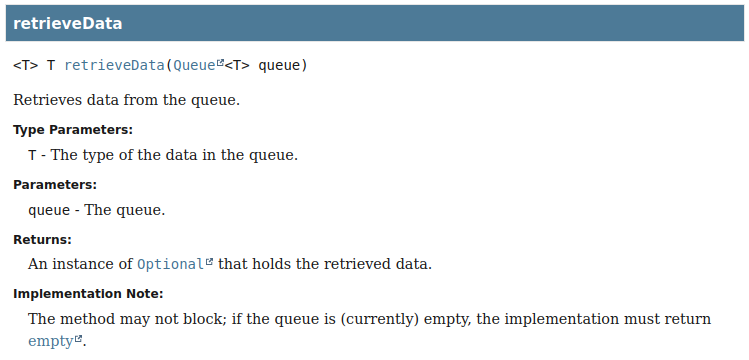
\includegraphics[scale=0.55]{comments/JavadocCustomTag1}
\end{center}

The colon (\bdq{:}) is always the separator. To include a colon in the tag name, escape it with a backslash. Omitting a value for \texttt{<header>} causes the name to be the heading, and if no location is specified, the tag can be used everywhere (same as \texttt{A} was specified). Refer also to \autocite{ORACLE_DOC_JAVADOC_MAN:StandardDocletOptions}.

The three tags below are defined per convention and widely used throughout the official documentation of the \Java API:

\paragraph{\lstinline|@apiNote|}\label{sec:TagApiNote}\index{apiNote@"@apiNote} Usage: \lstinline|@apiNote <text>|

This tag is used to provided some notes regarding the API.

\paragraph{\lstinline|@implNote|}\label{sec:TagImplNote}\index{implNote@"@implNote} Usage: \lstinline|@implNote <text>|

With this tag, you can add notes on how an implementation looks like (or should look like) to a program element.

\paragraph{\lstinline|@implSpec|}\label{sec:TagImplSpec}\index{implSpec@"@implSpec} Usage: \lstinline|@implSpec <text>|

This tag is added to provide information about the specification that is the base of the implementation for the respective program element.

\keeplisting{4}
To use these tags, they must be registered on the command line like this:
\begin{lstlisting}[numbers=none,language=sh]
javadoc -tag apiNote:a:API Note: \
        -tag implSpec:a:Implementation Requirements: \
        -tag implNote:a:Implementation Note:
\end{lstlisting}

%------------------------------------------------------------------------------

\subsubsection{Custom Taglets}\label{sec:CustomTaglets}
An introduction to implementing custom taglets would go beyond the scope of this book. However, the documentation for the \lstinline|jdk.javadoc.doclet.Taglet|\index{jdk.javadoc.doclet!Taglet} \autocite{ORACLE_DOC_TAGLET_INTERFACE} already provides a useful starting point.

Custom taglets do allow also the implementation of inline tags, on the other hand, they do not support to include the already existing inline tags.

If you want to use custom taglets, you have to provide the path to the implementing classes with the command line option \mbox{\texttt{-tagletpath}}; multiple locations are separated by a colon (\bdq{:}) on Linux/Unix operating systems, or by a semi-colon (\bdq{;}) on Windows.

Next each Taglet implementation class needs to be registered with the command line option \mbox{\texttt{-tagletclass}} (one entry per class).

I created a set of custom tags that I use regularly, and that I also recommend for your documentation comments. The respective library (\bdq{tquadrat’s Javadoc Extensions} or short \bsq{foundation-javadoc}) can be found at \autocite{TQUADRAT_ORG_FOUNDATION_JAVADOC}.

The command line for this would look like this:\footnote{Check the project's website at \autocite{TQUADRAT_ORG_FOUNDATION_JAVADOC} for the current version.}
\keeplisting{20}
\begin{lstlisting}
-tagletpath /path/to/org.tquadrat.foundation.javadoc-0.25.4.jar:\
/path/to/apiguardian-api-1.1.2.jar:/path/to/jakarta.activation-2.0.1.jar \
\
-taglet org.tquadrat.foundation.javadoc.AnchorTaglet \
-taglet org.tquadrat.foundation.javadoc.AuthorTaglet \
-taglet org.tquadrat.foundation.javadoc.FALSETaglet \
-taglet org.tquadrat.foundation.javadoc.HRefTaglet \
-taglet org.tquadrat.foundation.javadoc.IgnoreTaglet \
-taglet org.tquadrat.foundation.javadoc.ImageTaglet \
-taglet org.tquadrat.foundation.javadoc.IncludeTaglet \
-taglet org.tquadrat.foundation.javadoc.InspiredTaglet \
-taglet org.tquadrat.foundation.javadoc.ModifiedTaglet \
-taglet org.tquadrat.foundation.javadoc.NoteTaglet \
-taglet org.tquadrat.foundation.javadoc.NULLTaglet \
-taglet org.tquadrat.foundation.javadoc.ThanksTaglet \
-taglet org.tquadrat.foundation.javadoc.ToDoTaglet \
-taglet org.tquadrat.foundation.javadoc.TRUETaglet \
-taglet org.tquadrat.foundation.javadoc.UmlGraphLinkTaglet \
-taglet org.tquadrat.foundation.javadoc.UnderlineTaglet \
\
-tag hidden -tag note -tag param -tag return -tag throws -tag author -tag extauthor -tag thanks -tag modified -tag version -tag since -tag see -tag inspired -tag spec -tag provides -tag uses -tag UMLGraph.link -tag deprecated -tag todo \
-tag apiNote:a:API Note: \ 
-tag implSpec:a:Implementation Requirements: \
-tag implNote:a:Implementation Note: 
\end{lstlisting}

The purpose of the \texttt{-tag} options here is to determine the order in which the block tags appear in the final documentation. The command line for the Javadoc\index{javadoc} tool is further discussed in chapter \tqfullref{sec:RunJavadoc}.

\bdq{tquadrat’s Javadoc Extensions} provides the following custom taglets:

\keeplisting{4}
\paragraph{\lstinline|@anchor|}\label{sec:TagAnchor}  Usage: \lstinline|{@anchor #<anchor-name> <text>}|

This tag allows to add an HTML anchor to the generated documentation, where \texttt{\#<anchor-name>} is the name of the anchor to the given text. The hash symbol (\bsq{\#}) before the name of the anchor is mandatory!

%------------------------------------------------------------------------------

\keeplisting{5}
\paragraph{\lstinline|@author|}\label{sec:TagExtAuthor}  Usage: \lstinline|@author <name-text> - <email-address>| or \\
\lstinline|    @extauthor <name-text> - <email-address>|

This is a replacement for the \nameref{sec:TagAuthor}\index{author@"@author} tag that renders the given email address as a \texttt{mailto:} link in the generated documentation. It does not regard the option \mbox{\texttt{-author}} on the command line\footnote{This is valid for the current version 0.25.4 of the library; it may have changed for a later version.}.

The \lstinline|@extauthor| was introduced because some versions of the Javadoc\index{javadoc} did not allow to overwrite the standard \nameref{sec:TagAuthor}\index{author@"@author} tag.

%------------------------------------------------------------------------------

\paragraph{\lstinline|@false|}\label{sec:TagFALSE}  Usage: \lstinline|{@false}|

This is a shortcut for \lstinline|{@code false}|\index{code@"@code}.

%------------------------------------------------------------------------------

\paragraph{\lstinline|@href|}\label{sec:TagHref}  Usage: \lstinline|{@href <url> <text>}| or \lstinline|{@href <url>}|

With this tag, an HTML hyperlink can be added to the generated documentation; it will be placed inside the description text, but different from the \nameref{sec:TagLink} and \nameref{sec:TagLinkplain} tags, it allows to refer to arbitrary external resources, not only to other documented elements. Obviously, \texttt{<url>} is the target URL, while \texttt{<text>} is the clickable text. If the latter is omitted, the URL itself will be used instead.

%------------------------------------------------------------------------------

\paragraph{\lstinline|@ignore|}\label{sec:TagIgnore}  Usage: \lstinline|{@ignore <text>}|

With this tag text can be added to the documentation comment that is not shown in the generated documentation.

%------------------------------------------------------------------------------

\paragraph{\lstinline|@image|}\label{sec:TagImage}  Usage: \lstinline|{@image <url> <attributes>}|

The tag allows to add a picture to the generated documentation. \texttt{<url>} is the location of the image file, while \texttt{<attributes>} are HTML\index{HTML} attributes that are allowed for the \lstinline|<img>| tag.

%------------------------------------------------------------------------------

\paragraph{\lstinline|@include|}\label{sec:TagInclude}  Usage: \lstinline|{@include <source>:<process-mode>|

This tag allows you to include the contents of an external file in different ways, determined by the \texttt{<process-mode>}. It can be used to embed source code snippets into the documentation, but also to load text modules. 

\keeplisting{5}
Valid values for \texttt{<process-mode>} are:
\begin{itemize}[nosep]
	\item PLAIN
	\item ESCAPE
	\item MARKDOWN
	\item SOURCE
\end{itemize}

The code below includes the contents of the same file:
\keeplisting{8}
\begin{lstlisting}[language=Comment]
 …
 *  <hr>
 *  <p>{@include ${includes}/sample.html:PLAIN}</p>
 *  <hr>
 *  <p>{@include ${includes}/sample.html:ESCAPE}</p>
 *  <hr>
 *  <p>{@include ${includes}/sample.html:SOURCE}</p>
 *  <hr>
 …
\end{lstlisting}

For \bdq{\texttt{<process-mode> = PLAIN}} the output looks like this: 
\begin{center}
	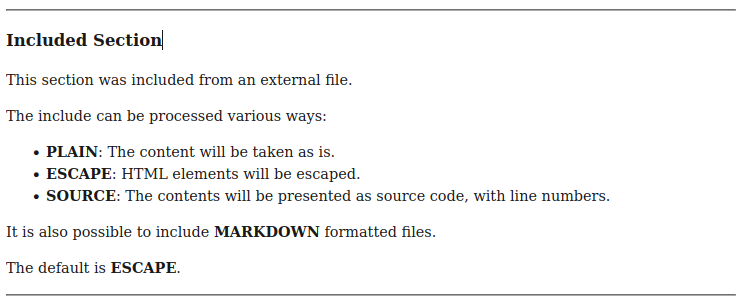
\includegraphics[scale=0.55]{comments/JavadocIncludePlain}
\end{center}
\bdq{\texttt{<process-mode> = ESCAPE}} is rendered like this: 
\begin{center}
	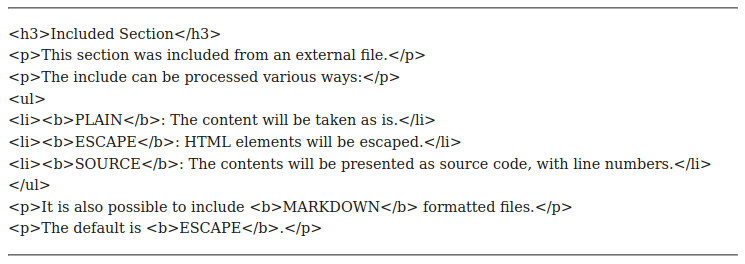
\includegraphics[scale=0.55]{comments/JavadocIncludeEscape}
\end{center}
And \bdq{\texttt{<process-mode> = SOURCE}} results a below: 
\begin{center}
	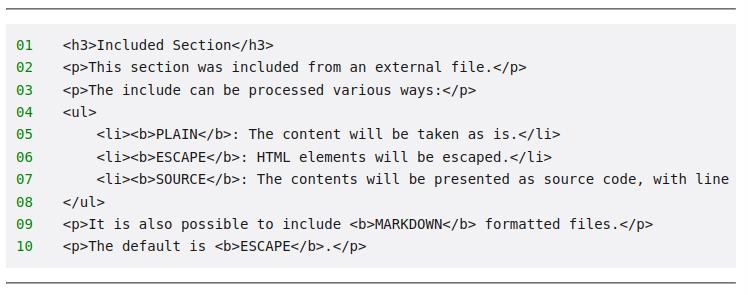
\includegraphics[scale=0.55]{comments/JavadocIncludeSource}
\end{center}

For more details on the \bdq{\{\nameref{sec:TagInclude}\}} tag, refer to \autocite{TQUADRAT_ORG_FOUNDATION_JAVADOC}.

%------------------------------------------------------------------------------

\paragraph{\lstinline|@inspired|}\label{sec:TagInspired}  Usage: \lstinline|@inspired <text>|

Sometimes a piece of code was inspired by a document of some kind, a description of an algorithm, a product white paper, or whatever. This tag allows you to add a reference to that source of inspiration.

Refer also to \nameref{sec:TagSpec}\index{spec@"@spec}, \nameref{sec:TagImplNote}\index{implNote@"@implNote}, \nameref{sec:TagImplSpec}\index{implSpec@"@implSpec} and \nameref{sec:TagApiNote}\index{apiNote@"@apiNote} as they are somehow related. In particular if the reference to the inspiration is only a URL, the \nameref{sec:TagSpec}\index{spec@"@spec} is preferred.

%------------------------------------------------------------------------------

\paragraph{\lstinline|@modified|}\label{sec:TagModified}  Usage: \lstinline|@modified <name-text> - <email-address>|

This is a variant of the \nameref{sec:TagExtAuthor} tag. It is meant to provide the name of the developer that modified the respective element without claiming to be an author.

%------------------------------------------------------------------------------

\paragraph{\lstinline|@note|}\label{sec:TagNote}  Usage: \lstinline|@note <text>|

With this tag, it is easy to add important notes to the generated documentation for an element. All notes will be added to a bullet list placed immediately beneath the documentation text. The text for the \lstinline|@note| tag is somehow limited as it does not allow other Javadoc tags.

%------------------------------------------------------------------------------

\paragraph{\lstinline|@null|}\label{sec:TagNULL}  Usage: \lstinline|{@null}|

This is a shortcut for \lstinline|{@code null}|\index{code@"@code}.

%------------------------------------------------------------------------------

\paragraph{\lstinline|@thanks|}\label{sec:TagThanks}  Usage: \lstinline|@thanks <name-text> - <email-address>|

Use this tag to mention someone who provided input to the respective element without being an author; that person might have wrote an article about the algorithm that was implemented by this element, or they may have reported a bug.

Same as for the \nameref{sec:TagExtAuthor} and the \nameref{sec:TagModified} tags, the email address will be rendered to a \verb#mailto:# link in the generated documentation.

%------------------------------------------------------------------------------

\paragraph{\lstinline|@todo|}\label{sec:TagTodo}  Usage: \lstinline|@todo <todo.md>|

This tag copies the contents of the Markdown\index{Markdown} file specified by \texttt{<todo.md>} into the generated documentation. This is meant as a ToDo list or list of open issues, and that is reflected by the heading that is added to the generated documentation.

%------------------------------------------------------------------------------

\paragraph{\lstinline|@true|}\label{sec:TagTRUE}  Usage: \lstinline|{@true}|

This is a shortcut for \lstinline|{@code true}|\index{code@"@code}.

%------------------------------------------------------------------------------

\paragraph{\lstinline|@UMLGraph.link|}\label{sec:TagUMLGraph}  Usage: \lstinline|@UMLGraph.link|

This adds an UML graph for the current class to the generated documentation.

%------------------------------------------------------------------------------

\paragraph{\lstinline|@underline|}\label{sec:TagUnderline}  Usage: \lstinline|{@underline <text>}|

Use this tag to add underlined text to the generated documentation.

%==============================================================================
% End of file!!
%==============================================================================



%==============================================================================
% End of file!!
%==============================================================================

